\reviewexercisesheader{}

% 39 - tf_correlation

\eoce{\qt{True / False\label{tf_correlation}}
Determine if the following statements are true or false.
If false, explain why.
\begin{parts}
\item A correlation coefficient of -0.90 indicates a stronger 
linear relationship than a correlation of 0.5.
\item Correlation is a measure of the association between any 
two variables.
\end{parts}
}{}

% 40 - cat_body_heart_inf_2s

\eoce{\qt{Cats, Part II\label{cat_body_heart_inf}}
Exercise~\ref{cat_body_heart_reg} 
presents regression output from a model for predicting the heart 
weight (in g) of cats from their body weight (in kg). The coefficients 
are estimated using a dataset of 144 domestic cat. The model output 
is also provided below.  Assume that conditions for inference on the slope are met.
\begin{center}
\begin{tabular}{rrrrr}
    \hline
            & Estimate  & Std. Error    & t value   & Pr($>$$|$t$|$) \\ 
    \hline
(Intercept) & -0.357    & 0.692         & -0.515    & 0.607 \\ 
body wt     & 4.034     & 0.250         & 16.119    & 0.000 \\ 
    \hline
\end{tabular}
\[ s = 1.452 \qquad R^2 = 64.66\% \qquad R^2_{adj} = 64.41\% \]
\end{center}
\begin{parts}
\item We see that the point estimate for the slope is positive.
    What are the hypotheses for evaluating whether body weight is
    positively associated with heart weight in cats?
\item State the conclusion of the hypothesis test from part (a) in 
context of the data.
\item Calculate a 95\% confidence interval for the slope of body 
weight, and interpret it in context of the data.
\item Do your results from the hypothesis test and the confidence 
interval agree? Explain.
\end{parts}
}{}

% 41 - starbucks_cals_protein

\eoce{\qt{Nutrition at Starbucks, Part II\label{starbucks_cals_protein}} 
Exercise~\ref{starbucks_cals_carbos} introduced a data set on nutrition 
information on Starbucks food menu items. Based on the scatterplot 
and the residual plot provided, describe the relationship between the 
protein content and calories of these menu items, and determine if a 
simple linear model is appropriate to predict amount of protein from 
the number of calories.
\begin{center}
\tabspecial{tableau-starbucks-p2}{
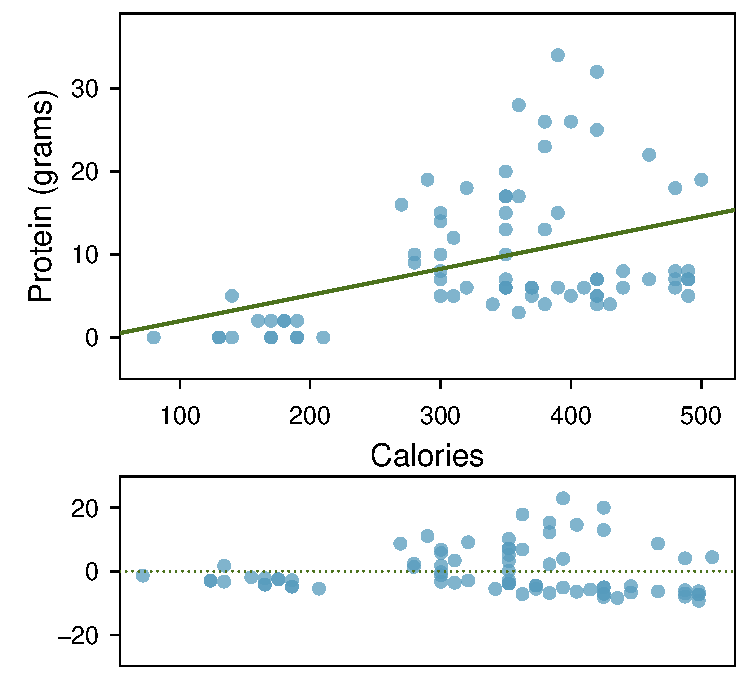
\includegraphics[width=0.35\textwidth]{ch_regr_simple_linear/figures/eoce/starbucks_cals_protein/starbucks_cals_protein}}
\end{center}
}{}

% 42 - helmet_lunch

\eoce{\qt{Helmets and lunches\label{helmet_lunch}}
The scatterplot shows the 
relationship between socioeconomic status measured as the percentage of 
children in a neighborhood receiving reduced-fee lunches at school 
({\tt lunch}) and the percentage of bike riders in the neighborhood 
wearing helmets ({\tt helmet}). The average percentage of children 
receiving reduced-fee lunches is 30.8\% with a standard deviation 
of 26.7\% and the average percentage of bike riders wearing helmets 
is 38.8\% with a standard deviation of 16.9\%.

\noindent\begin{minipage}[c]{0.5\textwidth}
{\raggedright\begin{parts}
\item If the $R^2$ for the least-squares regression line for these 
data is $72\%$, what is the correlation between {\tt lunch} 
and {\tt helmet}?
\item Calculate the slope and intercept for the least-squares regression 
line for these data.
\item Interpret the intercept of the least-squares regression line in 
the context of the application.
\item Interpret the slope of the least-squares regression line in the 
context of the application.
\item What would the value of the residual be for a neighborhood where 
40\% of the children receive reduced-fee lunches and 40\% of the bike 
riders wear helmets? Interpret the meaning of this residual in the context 
of the application.
\end{parts}}
\end{minipage}
\begin{minipage}[c]{0.05\textwidth}
$\:$ \\
\end{minipage}
\begin{minipage}[c]{0.42\textwidth}
\begin{center}
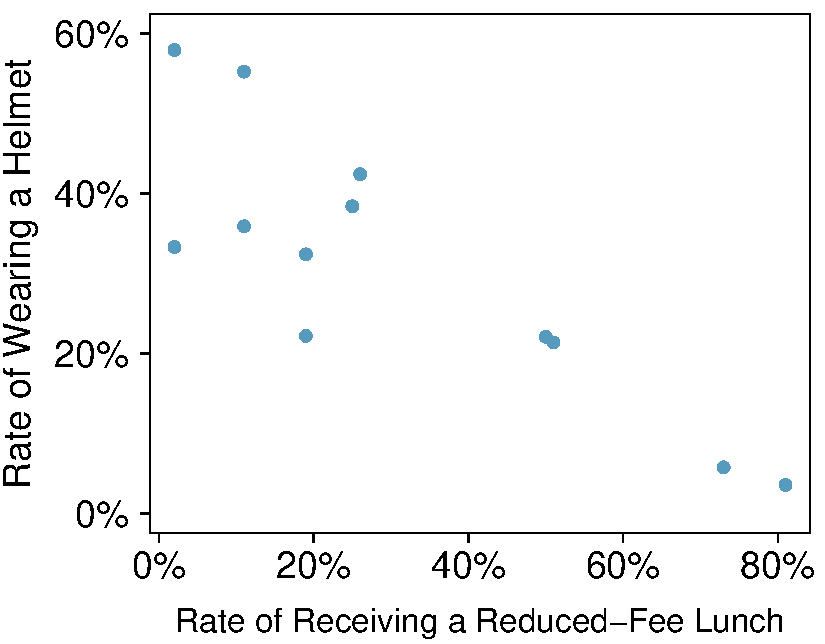
\includegraphics[width=\textwidth]{ch_regr_simple_linear/figures/eoce/helmet_lunch/helmet_lunch.pdf} \\
\end{center}
\end{minipage}
}{}

% 43 - match_corr_3

\eoce{\qt{Match the correlation, Part III\label{match_corr_3}} 
Match each correlation to the corresponding scatterplot.

\noindent%
\begin{minipage}[c]{0.17\textwidth}
\begin{parts}
\item $r = -0.72$
\item $r = 0.07$ 
\item $r = 0.86$ 
\item $r = 0.99$
\end{parts}\vspace{3mm}
\end{minipage}%
\begin{minipage}[c]{0.83\textwidth}
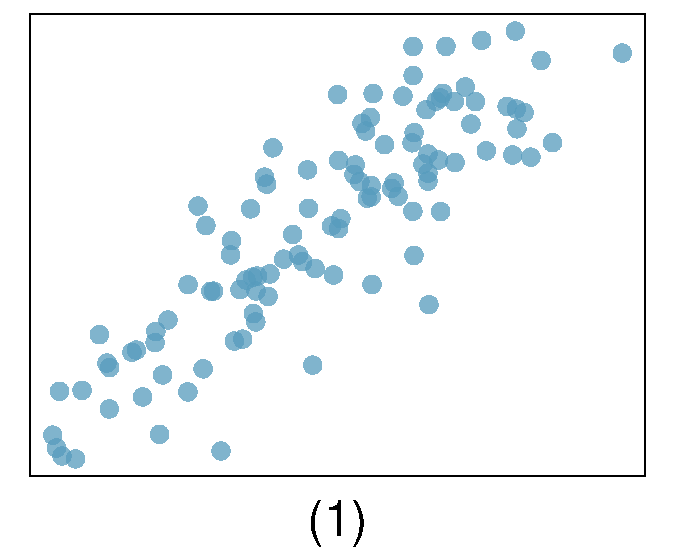
\includegraphics[width=0.245\textwidth]{ch_regr_simple_linear/figures/eoce/match_corr_3/scatter_1}
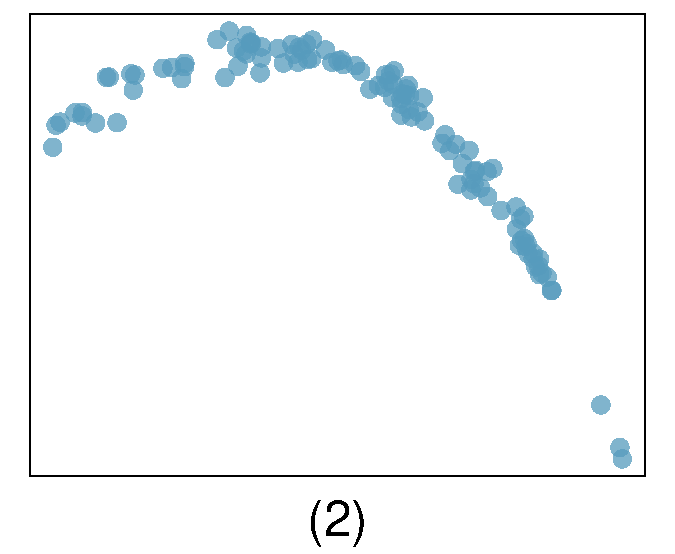
\includegraphics[width=0.245\textwidth]{ch_regr_simple_linear/figures/eoce/match_corr_3/scatter_2}
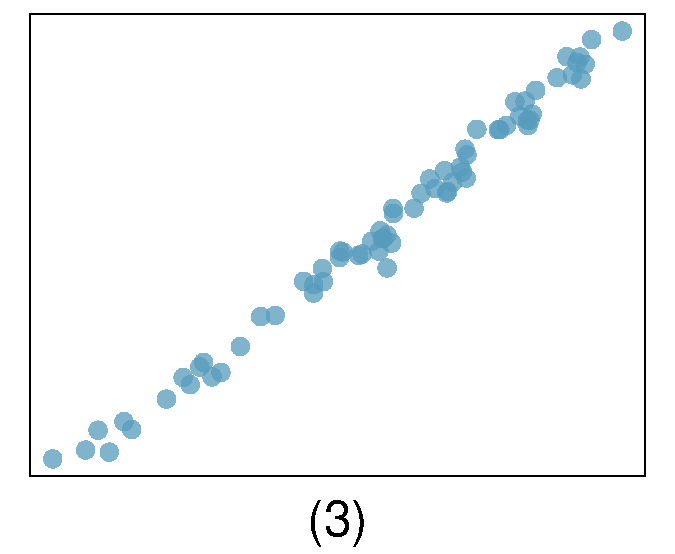
\includegraphics[width=0.245\textwidth]{ch_regr_simple_linear/figures/eoce/match_corr_3/scatter_3}
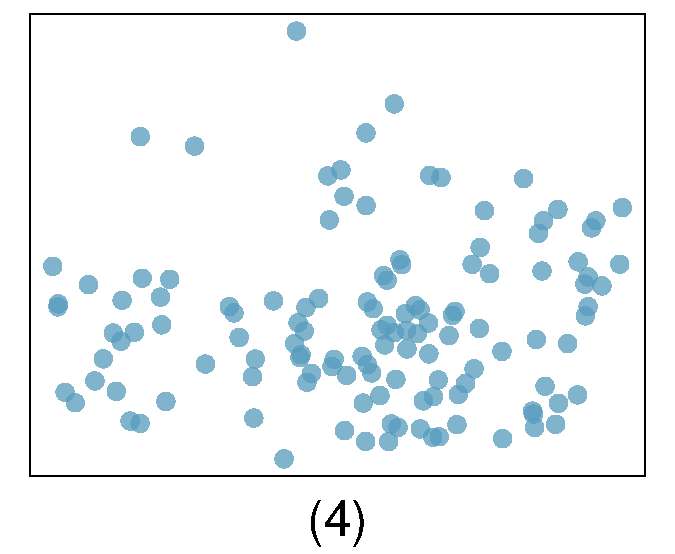
\includegraphics[width=0.245\textwidth]{ch_regr_simple_linear/figures/eoce/match_corr_3/scatter_4}
\end{minipage}
}{}

% 44 - rate_my_prof

\eoce{\qt{Rate my professor\label{rate_my_prof}}
Many college courses conclude by giving students
the opportunity to evaluate the course and the
instructor anonymously.
However, the use of these student evaluations
as an indicator of course quality and teaching
effectiveness is often criticized because these
measures may reflect the influence of
non-teaching related characteristics,
such as the physical appearance of the instructor.
Researchers at University of Texas, Austin
collected data on teaching evaluation score
(higher score means better) and standardized
beauty score (a score of 0 means average, negative
score means below average, and a positive score
means above average) for a sample of 463
professors.\footfullcite{Hamermesh:2005}
The scatterplot below shows the relationship
between these variables, and regression output
is provided for predicting teaching evaluation
score from beauty score.
\begin{center}
\begin{tabular}{rrrrr}
    \hline
            & Estimate  & Std. Error    & t value   & Pr($>$$|$t$|$) \\ 
  \hline
(Intercept) & 4.010     & 0.0255        & 	157.21  & 0.0000 \\ 
beauty      &  \fbox{\textcolor{white}{{\footnotesize Cell 1}}}  
                        & 0.0322        & 4.13      & 0.0000\vspace{0.8mm} \\ 
   \hline
\end{tabular}
\end{center}
\noindent\begin{minipage}[c]{0.45\textwidth}
{\raggedright\begin{parts}
\item
    Given that the average standardized beauty score
    is -0.0883 and average teaching evaluation score
    is 3.9983, calculate the slope.
    Alternatively, the slope may be computed using just
    the information provided in the model summary table.
\item
    Do these data provide convincing evidence that the
    slope of the relationship between teaching evaluation
    and beauty is positive?
    Explain your reasoning.
\item
    List the conditions required for linear regression
    and check if each one is satisfied for this model
    based on the following diagnostic plots.
\end{parts}}
\end{minipage}
\begin{minipage}[c]{0.07\textwidth}
$\:$ \\
\end{minipage}
\begin{minipage}[c]{0.45\textwidth}
\tabspecial{tableau-teaching-eval-beauty}{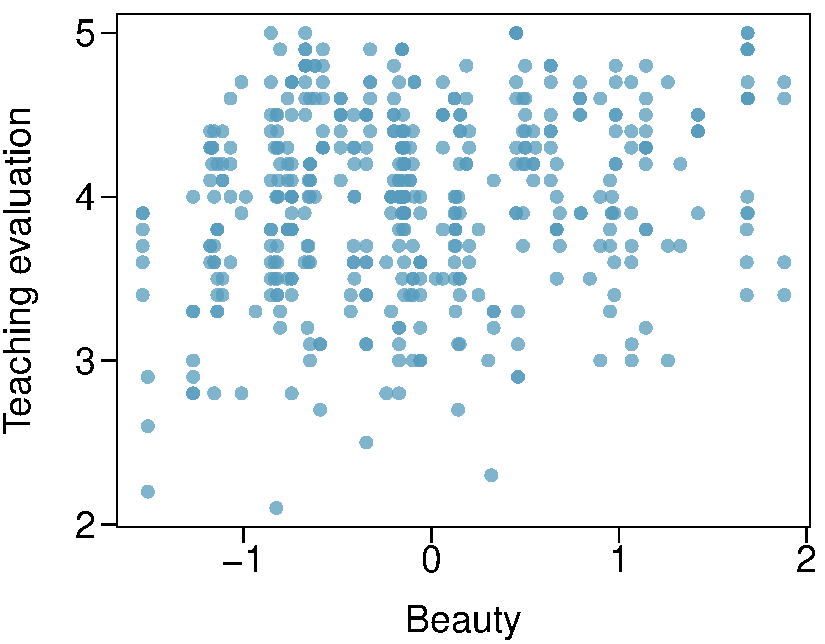
\includegraphics[width=\textwidth]{ch_regr_simple_linear/figures/eoce/rate_my_prof/rate_my_prof_eval_beauty.pdf}} \\
\end{minipage}
\begin{center}
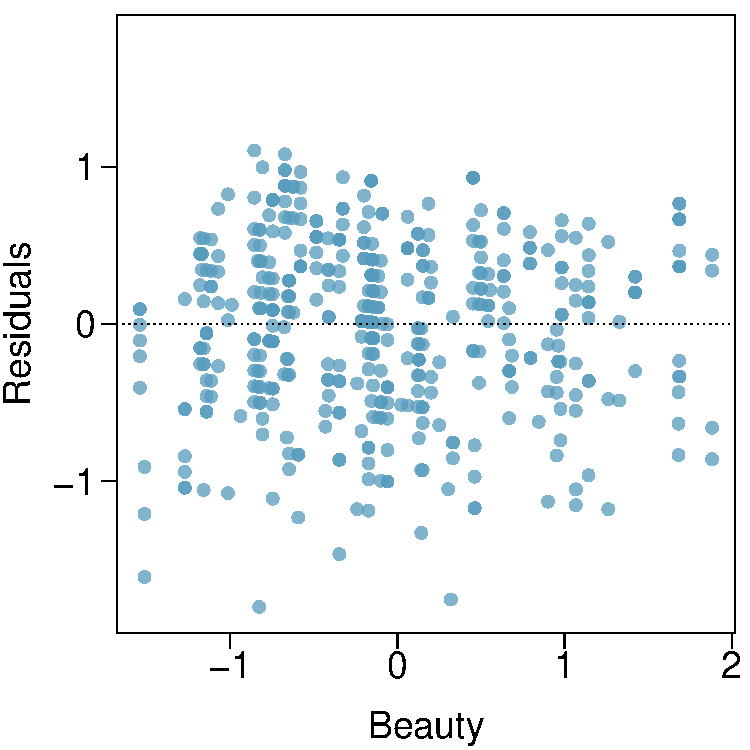
\includegraphics[width=0.32\textwidth]{ch_regr_simple_linear/figures/eoce/rate_my_prof/rate_my_prof_residuals}
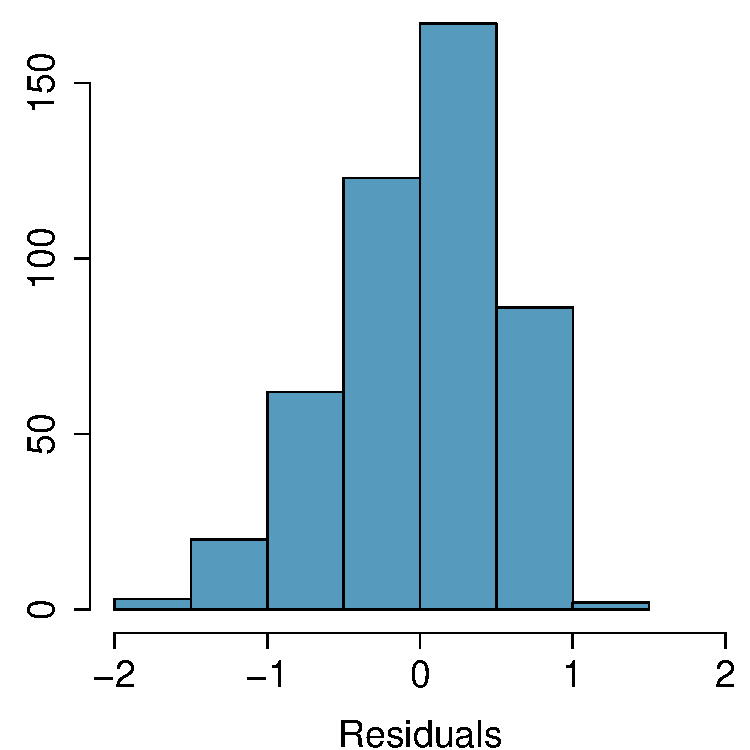
\includegraphics[width=0.32\textwidth]{ch_regr_simple_linear/figures/eoce/rate_my_prof/rate_my_prof_residuals_hist}
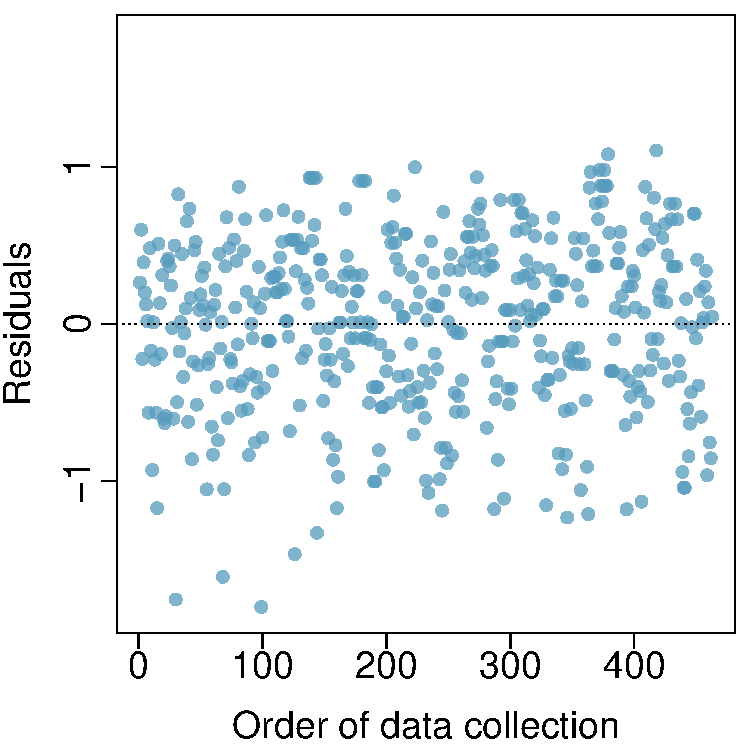
\includegraphics[width=0.32\textwidth]{ch_regr_simple_linear/figures/eoce/rate_my_prof/rate_my_prof_residuals_order}
\end{center}
}{}

\D{\newpage}
% 45 - trees_volume_height_diameter

\eoce{\qt{Trees\label{trees_volume_height_diameter}} The scatterplots below 
show the relationship between height, diameter, and volume of timber 
in 31 felled black cherry trees. The diameter of the tree is measured 
4.5 feet above the ground.\footfullcite{data:trees}
\begin{center}
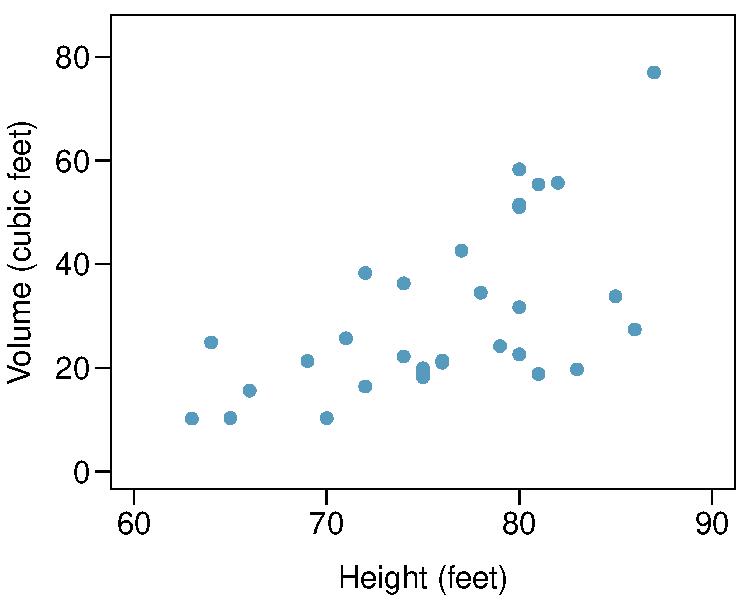
\includegraphics[width=0.46\textwidth]{ch_regr_simple_linear/figures/eoce/trees_volume_height_diameter/trees_volume_height.pdf}
\hspace{0.07\textwidth}%
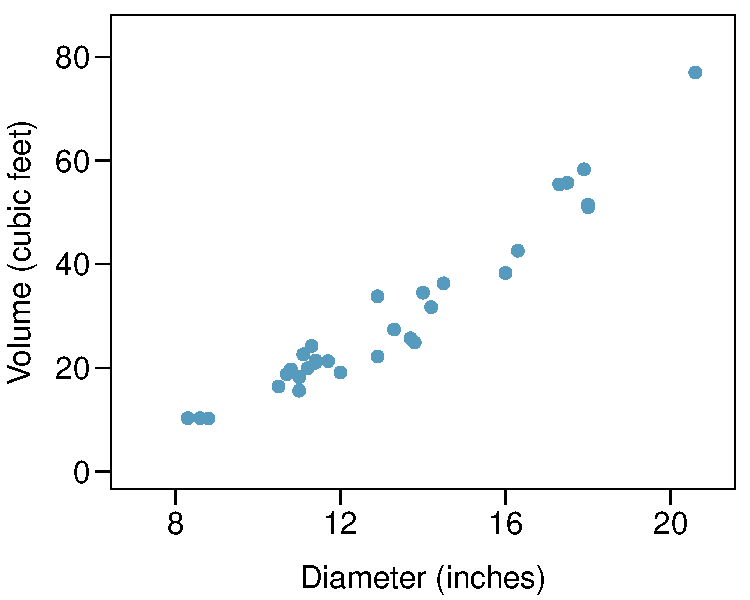
\includegraphics[width=0.46\textwidth]{ch_regr_simple_linear/figures/eoce/trees_volume_height_diameter/trees_volume_diameter.pdf}
\end{center}
\begin{parts}
\item Describe the relationship between volume and height of these trees.
\item Describe the relationship between volume and diameter of these trees.
\item Suppose you have height and diameter measurements for another black 
cherry tree. Which of these variables would be preferable to use to predict 
the volume of timber in this tree using a simple linear regression model? 
Explain your reasoning.
\end{parts}
}{}
